%++++++++++++++++++++++++++++++++++++++++
\documentclass[article, 12pt]{article}
\usepackage{float}
\usepackage{setspace}
\usepackage{tabu} % extra features for tabular environment
\usepackage{amsmath}  % improve math presentation
\usepackage{graphicx} % takes care of graphic including machinery
\usepackage[margin=1in]{geometry} % decreases margins
\usepackage{cite} % takes care of citations
\usepackage[final]{hyperref} % adds hyper links inside the generated pdf file
\usepackage{tikz}
\usepackage{caption} 
\usepackage{fancyhdr}
\usepackage{amssymb} % symbols like /therefore
\usepackage{amsthm} % proofs
\usepackage{enumerate} % lettered lists
\usepackage{mathtools} % macros
\usepackage{stix}
\usetikzlibrary{scopes}
% \usepackage{xcolor} \pagecolor[rgb]{0.12549019607,0.1294117647,0.13725490196} \color[rgb]{0.82352941176,0.76862745098,0.62745098039} % dark theme
\theoremstyle{definition}
\newtheorem{example}{Example}[subsubsection]
\newtheorem*{remark}{Remark}
\newtheorem{theorem}{Theorem}[subsubsection]
\newtheorem{definition}{Definition}[subsubsection]
\newtheorem{corollary}{Corollary}[subsubsection]
\hypersetup{
	colorlinks=false,      % false: boxed links; true: colored links
	linkcolor=blue,        % color of internal links
	citecolor=blue,        % color of links to bibliography
	filecolor=magenta,     % color of file links
	urlcolor=blue         
}
\usepackage{physics}
\usepackage{siunitx}
\usepackage{tikz,pgfplots}
\usepackage[outline]{contour} % glow around text
\usetikzlibrary{calc}
\usetikzlibrary{angles,quotes} % for pic
\usetikzlibrary{arrows.meta}
\tikzset{>=latex} % for LaTeX arrow head
\contourlength{1.2pt}

\colorlet{xcol}{blue!70!black}
\colorlet{vcol}{green!60!black}
\colorlet{myred}{red!70!black}
\colorlet{myblue}{blue!70!black}
\colorlet{mygreen}{green!70!black}
\colorlet{mydarkred}{myred!70!black}
\colorlet{mydarkblue}{myblue!60!black}
\colorlet{mydarkgreen}{mygreen!60!black}
\colorlet{acol}{red!50!blue!80!black!80}    
\tikzstyle{CM}=[red!40!black,fill=red!80!black!80]
\tikzstyle{xline}=[xcol,thick,smooth]
\tikzstyle{mass}=[line width=0.6,red!30!black,fill=red!40!black!10,rounded corners=1,
                  top color=red!40!black!20,bottom color=red!40!black!10,shading angle=20]
\tikzstyle{faded mass}=[dashed,line width=0.1,red!30!black!40,fill=red!40!black!10,rounded corners=1,
                        top color=red!40!black!10,bottom color=red!40!black!10,shading angle=20]
\tikzstyle{rope}=[brown!70!black,very thick,line cap=round]
\def\rope#1{ \draw[black,line width=1.4] #1; \draw[rope,line width=1.1] #1; }
\tikzstyle{force}=[->,myred,very thick,line cap=round]
\tikzstyle{velocity}=[->,vcol,very thick,line cap=round]
\tikzstyle{Fproj}=[force,myred!40]
\tikzstyle{myarr}=[-{Latex[length=3,width=2]},thin]
\def\tick#1#2{\draw[thick] (#1)++(#2:0.12) --++ (#2-180:0.24)}
\DeclareMathOperator{\sn}{sn}
\DeclareMathOperator{\cn}{cn}
\DeclareMathOperator{\dn}{dn}
\def\N{80} % number of samples in plots


\usepackage{titling}
\renewcommand\maketitlehooka{\null\mbox{}\vfill}
\renewcommand\maketitlehookd{\vfill\null}
\usepackage{siunitx} % units
\usepackage{verbatim} 
\newcommand{\courseNumber}{MATH 1700}
\newcommand{\courseName}{Ideas in Mathematics}
\newcommand{\professor}{Professor Rimmer}
\newcommand{\psetName}{Worksheet 1: The Pigeonhole Principle Second Submission}
\newcommand{\name}{Denny Cao}
\pagestyle{fancy}
\fancyhf{}% clears all header and footer fields
\fancyfoot[C]{--~\thepage~--}
\renewcommand*{\headrulewidth}{0.4pt}
\renewcommand*{\footrulewidth}{0pt}
\lhead{\name}
\chead{\courseNumber: \courseName}
\rhead{\professor}


\fancypagestyle{plain}{%
  \fancyhf{}% clears all header and footer fields
  \fancyfoot[C]{--~\thepage~--}%
  \renewcommand*{\headrulewidth}{0pt}%
  \renewcommand*{\footrulewidth}{0pt}%
}

% Shortcuts
\DeclarePairedDelimiter\ceil{\lceil}{\rceil} % ceil function
\DeclarePairedDelimiter\floor{\lfloor}{\rfloor} % floor function

\DeclarePairedDelimiter\paren{(}{)} % parenthesis

\newcommand{\df}{\displaystyle\frac} % displaystyle fraction
\newcommand{\qeq}{\overset{?}{=}} % questionable equality

\newcommand{\Mod}[1]{\;\mathrm{mod}\; #1} % modulo operator

% Sets
\DeclarePairedDelimiter\set{\{}{\}}
\newcommand{\unite}{\cup}
\newcommand{\inter}{\cap}

\newcommand{\reals}{\mathbb{R}} % real numbers: textbook is Z^+ and 0
\newcommand{\ints}{\mathbb{Z}}
\newcommand{\nats}{\mathbb{N}}
\newcommand{\rats}{\mathbb{Q}}

\newcommand{\degree}{^\circ}

% Counting
\newcommand\perm[2][^n]{\prescript{#1\mkern-2.5mu}{}P_{#2}}
\newcommand\comb[2][^n]{\prescript{#1\mkern-0.5mu}{}C_{#2}}

\setlength\parindent{0pt}

% Sign Charts
\newdimen\tcolw \tcolw=2.5em % the column width
\edef\ecatcode{\catcode`&=\the\catcode`&\relax}\catcode`&=4
\def\sgchart#1#2{\vbox{\offinterlineskip\halign{\hfil##\quad&##\hfil\crcr\sgchartA#2,:,%
   \omit\sgchartR&\kern.2pt\sgchartS{.5\tcolw}\relax\sgchartE#1,\relax,%
   \sgchartS{.5\tcolw}\relax\cr
   \noalign{\kern2pt}&\def~{}\kern.5\tcolw\sgchartD#1,\relax,\cr}}}
\def\sgchartA#1:#2,{\cr\ifx,#1,\else $#1$&\sgchartB#2{}\expandafter\sgchartA\fi}
\def\sgchartB#1{\hbox to\tcolw{\hss$#1$\hss}\sgchartC}
\def\sgchartC#1{\ifx,#1,\else
   \strut\vrule\kern-.4pt\hbox to\tcolw{\hss$#1$\hss}\expandafter\sgchartC\fi}
\def\sgchartD#1#2,{\ifx\relax#1\else\hbox to\tcolw{\hss$#1#2$\hss}\expandafter\sgchartD\fi}
\def\sgchartE#1#2,{\ifx\relax#1\else
    \ifx~#1\sgchartS\tcolw\circ \else\sgchartS\tcolw\bullet\fi \expandafter\sgchartE\fi}
\def\sgchartR{\leaders\vrule height2.8pt depth-2.4pt\hfil}
\def\sgchartS#1#2{\hbox to#1{\kern-.2pt\sgchartR \ifx\relax#2\else
   \kern-.7pt$#2$\kern-.7pt\sgchartR\fi\kern-.2pt}}
\ecatcode
%++++++++++++++++++++++++++++++++++++++++
\title{
    \vspace{2in}
    \textmd{\textbf{\courseNumber: \courseName}}
    \normalsize\vspace{0.1in}\\
    \vspace{0.1in}\Large{\text{\psetName}} \\
    \vspace{0.1in}\large{\text{\professor}}
    \vspace{3in}
}

\author{\name}
\date{Due: January 23, 2023}

\begin{document}
    \maketitle
    \thispagestyle{empty}
    \pagebreak

    \section{Warm-Up Problems}
    \begin{enumerate}[(1)]
        \item \textbf{Penn has four undergraduate schools: Arts and Sciences (including LPS), Engineering,
        Nursing, Wharton. Explain why, if you know five Penn undergraduates, at least two of
        them must be enrolled in the same school. What are the pigeons? The pigeonholes?}
        \begin{proof}
            Let each school be a pigeonhole, and each student be a pigeon. Then, with 4 pigeonholes and 4 pigeons, it is possible for each pigeon can be placed in each pigeonhole; 4 is not enough pigeons to guarantee 2 pigeons in 1 pigeonhole. With an additional pigeon (5 students), there must be at least one pigeonhole with two pigeons. Therefore, with 5 Penn undergraduates, at least two students must be in the same school.
        \end{proof}
        \item \textbf{According to Wikipedia, in 2016 the combined average daily traffic for the Lincoln and
        Holland Tunnels (which connect New Jersey with Manhattan, under the Hudson River)
        was 112,995 vehicles. Explain why, on any day with roughly average traffic, at least one
        of the two tunnels must have carried over 56,000 vehicles. What are the pigeons? The
        pigeonholes?}
        \begin{proof}
            Let each tunnel be a pigeonhole, and each vehicle be a pigeon. With 112,000 vehicles---pigeons---and 2 tunnels---pigeonholes---it is possible for 56,000 vehicles to be in each tunnel. With an additional vehicle, there must be at least one tunnel with over 56,000 vehicles. As $112,995>56,000$, with 112,995 vehciles there must be at least one tunnel with over 56,000 vehicles.
        \end{proof}
        \item \textbf{The record low temperature in Philadelphia is about \SI{-12}{\degree} F. The record high is about \SI{107}{\degree}
        F. Explain why you can be reasonably confident that, to the nearest degree, there will be
        two days in 2022 that are the have the same temperature at noon. Is your conclusion still
        true if you work with exact temperatures instead of rounding to the nearest degree?}
        \begin{proof}
            Given the two extremes, we can reasonably conclude that the temperatures in Philadelphia at any given time will be between -12 and 107 degrees Fahrenheit, totalling to 119 distinct temperatures. Let each distinct temperature be a pigeonhole and each day a pigeon. With 119 days, each can have a unique temperature at noon. With 120, there must be another day that has the same temperature at noon as another date, as there are not enough distinct temperatures. Since there are 365 days in a year---which is greater than 120---there are at least two days that have the same temperature at noon.
        \end{proof}
        This will not be true if we work with exact temperatures. By using exact temperatures, there are an infinite amount of unique temperatures. Even when we round to the nearest tenth of a degree, there are 10 numbers between two integers, and thus there are $119 \cdot 10-9=1181$ distinct temperatures (The additional minus 9 is due to no numbers being greater than 119.0). With just 365 days, there are not enough days to guarentee that there are two days with the same temperature at noon, as each noon of each day can map to only one temperature in the 1181 pigeonholes, making it possible for each pigeon to be placed in a unique pigeonhole.
    \end{enumerate}
\section{More Challenging Questions}
\begin{enumerate}[(1)]
    \stepcounter{enumi}
    \stepcounter{enumi}
    \stepcounter{enumi}
    \item \textbf{Explain why, if you choose 5 distinct numbers from the set $\set*{1,2,3,4,5,6,7,8}$, two of these members must add up to 9.}
    \begin{proof}
        We can create tuples of the form $(a,b)$, where $a$ and $b$ are distinct numbers from the set $\set*{1,2,3,4,5,6,7,8}$ and $a+b=9$. The set of these tuples is: $\set*{(1,8),(2,7),(3,6),(4,5)}$. Let each tuple be a pigeonhole. With 4 distinct numbers---4 pigeons---we can place each pigeon in each pigeonhole. With another pigeon, there must be at least one pigeonhole with two pigeons---there must be two numbers that add up to 9. Thus, if you choose 5 distinct numbers from the set $\set*{1,2,3,4,5,6,7,8}$, two of these members must add up to 9.
    \end{proof}
    \item \textbf{15 children participate in an Easter Egg hunt. If they bring back a total of 100 eggs, must two of them bring back the same number of eggs? (You might be able to solve this without the pigeonhole principle.)}
    \begin{proof} Contradiction. Let $p$ be the proposition that the 15 children bring back a total of 100 eggs, and $q$ be the proposition that two of them bring back the same number of eggs. To prove $p \to q$, we assume the negation, $p \land \neg q$: \\

        If each child brings back the least amount of eggs possible, then child 1 brings back 0 eggs, child 2 brings back 1 egg, child 3 brings back 2 eggs, and so on:
        \[ 0,1,2,3, \dots, 14\]
        The total eggs brought back is:
        \[ \sum_{i=0}^{14} i = 105 \smashtimes \]
        We arrive at a contradiction, as the total eggs brought back is 105, which exceeds the 100 eggs that were brought back. Had the children brought back more eggs, the the total would have also exceeded 100. Thus, $p \to q$ is true, meaning that, if 15 children brought back a total of 100 eggs, then 2 of them must bring back the same number of eggs.
    \end{proof}
    \item \textbf{How many cards must you draw from a standard deck to ensure that you have at least 3 cards with the same number and another 2 cards with the same number? (For the purposes of this problem, we consider J, Q, K, and A to be “numbers.”)}
    \begin{proof}
        Let each pigeonhole represent a card, and each pigeon is a card drawn from the deck. With 13 cards, it is possible to place each card in each pigeonhole. With 26 cards, it is possible place 2 cards in each pigeonhole. With an additional card, there must be one pigeonhole with at least 3 cards. Thus, we must draw at least 27 cards to ensure that we have at least 3 cards with the same number. To guarentee 3 cards with the same number, the other pigeonholes contain 2 pigeons, so there are already another 2 cards with the same number. Thus, we must draw at least 27 cards to ensure that we have at least 3 cards with the same number and another 2 cards with the same number.
    \end{proof}
    \item \textbf{Suppose you have 8 distinct whole numbers. Why must it be possible to subtract two of them and end up with a multiple of 7? (Hint: how much do you need to subtract from each number to obtain a multiple of 7?)}
    \begin{proof}
        We can represent the situation of two numbers subtracted and the difference is a multiple of 7 as:
        \begin{equation*}
            (x_1 - x_2)\Mod{7} = (x_1\Mod{7}) - (x_2\Mod{7}) = 0
        \end{equation*}
        Let $S$ be the set of remainders when dividing by 7. $S = \set*{0,1,2,3,4,5,6}$. Let each remainder in the set be a pigeonhole. With 7 distinct numbers, it is possible to place each number in each pigeonhole. With an additional number, there must be at least one pigeonhole with two numbers; two numbers have the same remainder when divided by 7. As they have the same remainder, there will be no remainder when both are divided by 7 and then subtracted. Thus, with 8 distinct whole numbers, it is possible to subtract two of the numbers and end up with a multiple of 7.
    \end{proof}
    \item \textbf{(Adapted from the 1958 Putnam Exam) Show that if you select 6 numbers from the set $\set*{1, 2, 3, 4, 5, 6, 7, 8, 9, 10}$, one must be a multiple of another.}
    \begin{proof}
        Let $S$ be the set $\set*{1 \leq k \leq 10 \eval k \in \ints}$. We can create a set of tuples $(a,b)$, where $a$ and $b$ are distinct numbers from $S$ such that $b=ka, k \in \nats$. Let $P$ be the set of these tuples; $P = \set*{(1,7), (2,6), (3,9), (4,8), (5,10)}$. By selecting 5 numbers, it is possible to select one number from each tuple. By selecting 1 more number, we guarentee that at least one tuple is in $P$. Since $P$ is a set of tuples where one number is a multiple of another, if you select 6 numbers from the set $S$, one must be a multiple of another.
    \end{proof}
    \item \textbf{There are 9 points, inside an equilateral triangle, and no line passes through more than two of these points, which means that any three points are the corners of a triangle. Explain why it must be possible to find three of these points, so that the area of the triangle formed by those three has at most one fourth of the area of the original triangle.} \label{question:equilateral}
    \begin{proof}
        We can partition an equilateral triangle into 4 equal parts as shown:
        \begin{figure}[H]
            \centering
            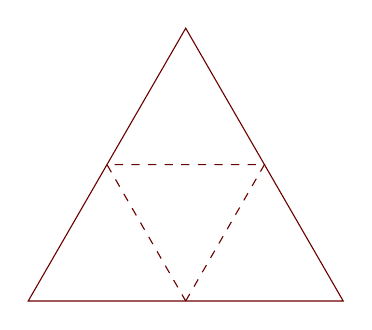
\begin{tikzpicture}
                \coordinate (A) at (0,0);
                \coordinate (B) at (4,0);
                \coordinate (C) at (2, {sin(60) * 4});
                
                % Midpoints
                \coordinate (AB) at ($(A)!0.5!(B)$);
                \coordinate (BC) at ($(B)!0.5!(C)$);
                \coordinate (CA) at ($(C)!0.5!(A)$);

                % Draw triangle ABC
                \draw[myred!60!black] (A) -- (B) -- (C) -- cycle;

                % Connect midpoints
                \draw[dashed, myred!60!black] (AB) -- (BC) -- (CA) -- cycle;
            \end{tikzpicture}
        \end{figure}
        As the area of the sections are the same, there is an equal probability that any point will be in each section. Let each smaller triangle be a pigeonhole, and each point a pigeon. With 8 points, it is possible for 2 points to be in each partition. With an additional point---9 total points---we guarantee that at least one section will have at least 3 points. The maximum area of these three points is the area of the partition triangle it belongs to, which is $\frac{1}{4}$ the area of the original triangle. Thus, with 9 points, it is possible to find three points so that the area of the triangle formed by those three has at most one fourth of the area of the original triangle.
    \end{proof}
\end{enumerate}
\section{Reflection}
\textbf{Identify at least one wrong or failed idea that turned out to be helpful or enlightening in some way. For instance, that idea might have helped you solve a problem, or it may have been the start of a conversation that improved your understanding more generally. You can list one of your own ideas, or an idea that originated with a classmate. (Please give your classmate credit!)} \\
For \hyperref[question:equilateral]{Question 9}, I discussed with a friend outside of class, Ethan. We formed a couple of ideas: inscribing a nonagon within the equilateral triangle, and somehow using Sierpinski's Triangle. Both of these ideas ended up being unsuccessful in solving the problem, but they were still helpful in the sense that they led to further conversations and brainstorming sessions that improved our understanding of the problem and the concept of geometric probability. The idea of inscribing a nonagon within the triangle led us to think about the relationship between the number of points and the area of the triangle they formed, which ultimately led to the solution I presented in my proof. Later on, I realized that I could use a first iteration Sierpinski's Triangle to partition the triangle into 4 even sectors---the basis of my proof. Even though these ideas did not directly solve the problem, they were still valuable in helping us understand the problem better and come up with a solution.
\end{document}
